\documentclass{standalone}
\usepackage{tikz}
\usepackage{tkz-fct}
\usepackage{tkz-euclide}



\begin{document}


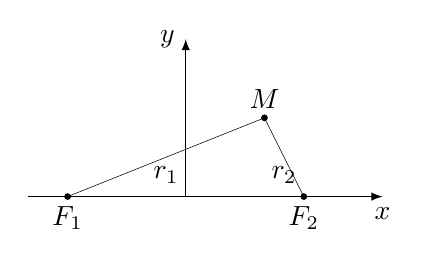
\begin{tikzpicture}
  \tkzInit[xmin=-2,xmax=2,ymin=0,ymax=1.5]
  \tkzDrawXY[noticks]
  %def points
  \tkzDefPoint(-1.5,0){F1}
  \tkzDefPoint(1.5,0){F2}
  \tkzDefPoint(1,1){M}
  %draw segments
  \tkzDrawSegments(F1,M M,F2)
  %label segments
  \tkzLabelSegment(F1,M){$r_1$}
  \tkzLabelSegment(M,F2){$r_2$}
  %draw points
  \tkzDrawPoints(F1,F2,M)
  %label points
  \tkzLabelPoint[below](F1){$F_1$}
  \tkzLabelPoint[below](F2){$F_2$}
  \tkzLabelPoint[above](M){$M$}
\end{tikzpicture}



\end{document}
